\section{Examples for a 3D Subduction Zone}
\label{sec:example:subduction:3d}

\subsection{Overview}

This suite of examples demonstrates use of a wide variety of features
and the general workflow often used in research simulations. We base
the model on the Cascadia subduction zone
(Figure~\ref{fig:example:subduction:3d:cascadia}). These examples will
focus on modeling the deformation associated with the the subducting
slab, including interseismic deformation with aseismic slip (creep)
and viscoelastic relaxation, coseismic slip on the slab interface and
a splay fault, and slow slip events on the top slab interface. We want
to account for the 3-D material properties associated with different
elastic properties for the subducting slab, mantle, continental crust,
and an accretionary wedge. To keep the computation time in these
examples short, we limit our model to an 800 km $\times$ 800 km
$\times$ 400 km domain and we will use a relatively coarse
discretization. For simplicity and to reduce complexity in constructing
the mesh, we use a flat top surface (elevation of 0 with respect
to mean sea level).

\begin{figure}[htbp]
  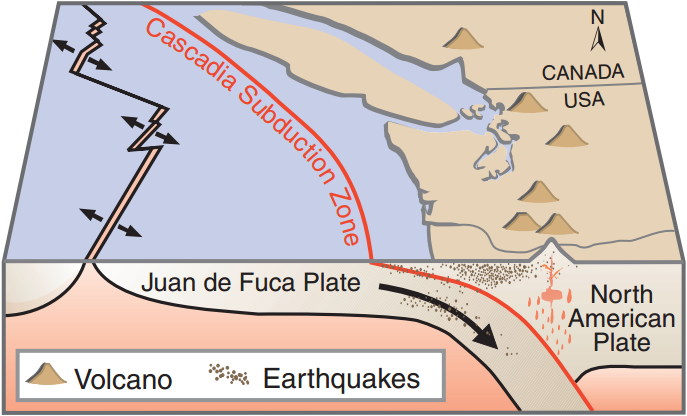
\includegraphics[width=4.5in]{examples/figs/subduction3d_cascadia}
  \caption{Cartoon of the Cascadia Subduction Zone showing the
    subduction of the Juan de Fuca Plate under the North American
    Plate. Source:
    \href{https://pubs.usgs.gov/fs/2000/fs060-00/}{U.S. Geological
      Survey Fact Sheet 060-00}}
  \label{fig:example:subduction:3d:cascadia}
\end{figure}

Figure~\ref{fig:example:subduction:3d:concept} shows our conceptual
model with a slab, mantle, continental crust, and accretionary
wedge. We cut off the slab at a depth of 100 km. We use a transverse
geographic projection coordinate system with Portland, Oregon, as the
origin in order to georeference our model. In order to model the
motion of the slab, we include a fault on the top of the slab at the
interface between the mantle, crust, and wedge, as well as a fault
between the bottom of the slab and the mantle.

\begin{figure}[htbp]
  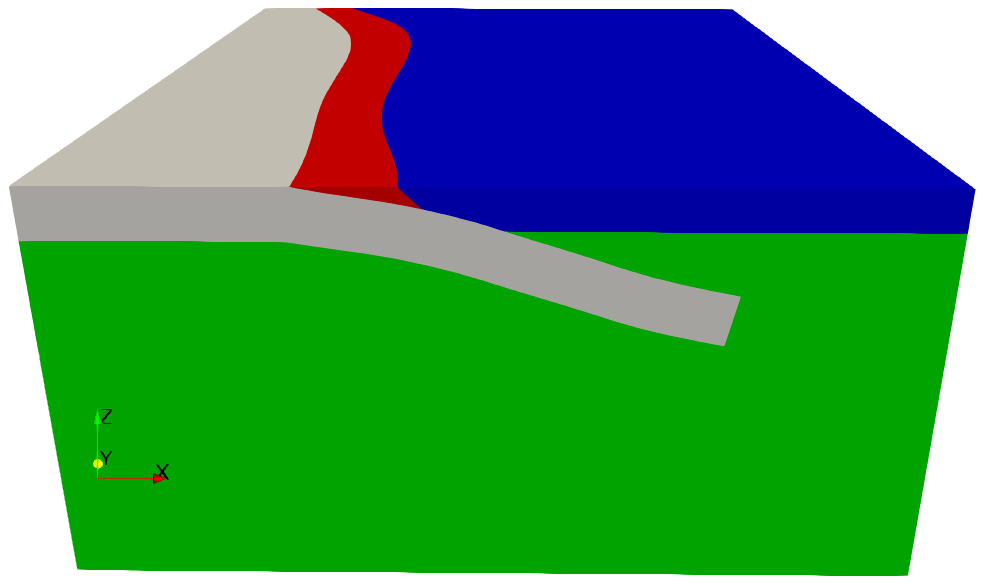
\includegraphics[width=4.5in]{examples/figs/subduction3d_conceptualmodel}
  \caption{Conceptual model based on the Cascadia Subduction Zone. The
    model includes the subduction slab (white), the mantle (green),
    continental crust (blue), and an acrretionary wedge (red).}
  \label{fig:example:subduction:3d:concept}
\end{figure}

The files associated with this suite of examples are contained in the
directory \filename{examples/3d/subduction}. This directory contains
several subdirectories:
\begin{description}
\item[\filename{mesh}] Files used to construct the finite-element mesh using
  CUBIT/Trelis.
\item[\filename{spatialdb}] Files associated with the spatial
  and temporal databases.
\item[\filename{viz}] ParaView
  Python scripts and other files for visualizing results.
\item[\filename{output}] Directory containing simulation
  output. It is created automatically when running the
  simulations.
\end{description}


\subsection{Features Illustrated}

Table~\ref{tab:example:subduction:3d:features} lists the features
discussed in each of these 3-D subduction zone examples. With the
intent of illustrating features used in research simulations, we use
HDF5 output and, we make extensive use the most efficient
implementations of spatial databases (UniformDB and SimpleGridDB). We
also use ParaView Python scripts for visualizing the output. These
scripts can be run within the ParaView GUI or outside the ParaView
GUI, although the interaction is limited to rotating, translating, and
zooming when run outside the ParaView GUI.

\begin{table}[htbp]
  \caption{PyLith features covered in the suite of 3-D subduction zone examples.}
  \label{tab:example:subduction:3d:features}
  \rowcolors{2}{yellow!30}{white}
\resizebox{\textwidth}{!}{%
\begin{tabular}{|l|%% Example
    *{8}c|% General
    *{3}c|% Solver
    *{5}c|% Spatial Database
}
\hline
\rowcolor{blue!10}
Example
& \multicolumn{8}{c|}{General}
& \multicolumn{3}{c|}{Solver}
& \multicolumn{5}{c|}{Spatial Database}
\\ 
%%%%
\hline
\rowcolor{blue!10}

% General
& \rlabel{Dimension}
& \rlabel{Coordinate system}
& \rlabel{Mesh generator}
& \rlabel{Cells}
& \rlabel{Refinement}
& \rlabel{Reordering}
& \rlabel{Problem type}
& \rlabel{Time dependence}
% Solver
& \rlabel{Solver}
& \rlabel{Preconditioner}
& \rlabel{Time stepping}
% Spatial Database
& \rlabel{Uniform}
& \rlabel{Simple}
& \rlabel{Simple grid}
& \rlabel{Composite}
& \rlabel{Time history}
\\
\hline
3d/subduction/step01
& 3 & Proj & CUBIT & Tet & & \yes & TD & S 
& L & ILU & 
& x2 & x4 & & & 
\\ \hline
3d/subduction/step02
& 3 & Proj & CUBIT & Tet & & \yes & TD & QS 
& L & ML+CUST & BE 
& x2 & x3 & x2 & x2 & 
\\ \hline
3d/subduction/step03
& 3 & Proj & CUBIT & Tet & & \yes & TD & QS 
& L & ML+CUST & BE 
& x4 & x3 & x2 & x2 & 
\\ \hline
3d/subduction/step04
& 3 & Proj & CUBIT & Tet & & \yes & TD & QS 
& L & ML+CUST & BE 
& x7 & x3 & x5 & x2 & 
\\ \hline
3d/subduction/step05
& 3 & Proj & CUBIT & Tet & & \yes & TD & QS 
& NL & ML+CUST & BE 
& x7 & x3 & x5 & x2 & 
\\ \hline
3d/subduction/step06
& 3 & Proj & CUBIT & Tet & & \yes & TD & QS 
& NL & ML+CUST & BE 
& x1 & x4 & x1 & & x1 
\\ \hline
\end{tabular}}
\par
{\bf Problem type} -- TD: time dependent, GF: Green's functions. {\bf Time dependence} -- S: static, QS: quasi-static, D: dynamic. {\bf Solver} -- L: linear, NL: nonlinear. {\bf Preconditioner} -- ILU: ILU, ASM: Additive Schwarz, SCHUR: Schur complement, CUST: custom, ML: ML algebraic multigrid, GAMG: geometric algebraic multigrid. {\bf Time stepping} -- BE: Backward Euler, FE: Forward Euler. \\ 
\rowcolors{2}{yellow!30}{white}
\resizebox{\textwidth}{!}{%
\begin{tabular}{|l|%% Example
    *{4}c|% Boundary Condition
    *{8}c|% Fault
    *{9}c|% Bulk Rheology
    *{7}c|% Output
}
\hline
\rowcolor{blue!10}
Example
& \multicolumn{4}{c|}{Boundary Condition}
& \multicolumn{8}{c|}{Fault}
& \multicolumn{9}{c|}{Bulk Rheology}
& \multicolumn{7}{c|}{Output}
\\ 
%%%%
\hline
\rowcolor{blue!10}

% Boundary Condition
& \rlabel{Dirichlet}
& \rlabel{Neumann}
& \rlabel{Absorbing}
& \rlabel{Point force}
% Fault
& \rlabel{Prescribed slip}
& \rlabel{Slip time function}
& \rlabel{Constitutive model}
& \rlabel{Static friction}
& \rlabel{Slip-weakening friction}
& \rlabel{Time-weakening friction}
& \rlabel{Rate-state friction w/ageing}
& \rlabel{Traction perturbation}
% Bulk Rheology
& \rlabel{Linear elastic}
& \rlabel{Linear Maxwell viscoelastic}
& \rlabel{Generalized Maxwell viscoelastic}
& \rlabel{Powerlaw viscoelastic}
& \rlabel{Drucker-Prager elastoplastic}
& \rlabel{Stress/strain formulation}
& \rlabel{Inertia}
& \rlabel{Reference state}
& \rlabel{Gravity}
% Output
& \rlabel{Format}
& \rlabel{Domain output}
& \rlabel{Surface output}
& \rlabel{Point output}
& \rlabel{State variable output}
& \rlabel{ParaView}
& \rlabel{Matplotlib}
\\
\hline
3d/subduction/step01
& x5 & & & 
& & & & & & & & & x4 & & & & & Inf & & & 
& H5 & x1 & x1 & & x4 & \yes & 
\\ \hline
3d/subduction/step02
& x5 & & & 
& x1 & STEP & & & & & & 
& x2 & x2 & & & & Inf & & & 
& H5 & x1 & x1 & & x4 & \yes & 
\\ \hline
3d/subduction/step03
& x5 & & & 
& x2 & RATE & & & & & & 
& x2 & x2 & & & & Inf & & & 
& H5 & x1 & x1 & & x4 & \yes & 
\\ \hline
3d/subduction/step04
& x5 & & & 
& x3 & STEP & & & & & & 
& x2 & x2 & & & & Inf & & & 
& H5 & x1 & x1 & & x4 & \yes & 
\\ \hline
3d/subduction/step05
& x5 & & & 
& x1 & RATE & x1 & & \yes & & & \yes 
& x2 & x2 & & & & Inf & & & 
& H5 & x1 & x1 & & x4 & \yes & 
\\ \hline
3d/subduction/step06
& x5 & & & 
& x1 & USER & & & & & & 
& x4 & & & & & Inf & & & 
& H5 & x1 & x1 & x1 & x4 & \yes & 
\\ \hline
\end{tabular}}
\par
{\bf Stress/strain formulation} -- Inf: infinitesimal, Fin: small, finite strain. \\ 

\end{table}

\subsection{Generating the Finite-Element Mesh}

We use CUBIT/Trelis to generate the finite-element mesh. Due to its
size, we do not include the finite-element mesh in the PyLith source
or binary distributions. If you do not have CUBIT/Trelis, you can
download the mesh from
\url{https://wiki.geodynamics.org/software:pylith:examples:files} and
skip generating the mesh.

We use contours of the Cascadia Subduction Zone from Slab v1.0
\ref{Hayes:etal:2012} for the geometry of the top of the slab. In
order to make use of these contours from within CUBIT/Trelis, we use a
Python script (\filename{generate\_surfjou.py}) to read the contours
file and create a CUBIT/Trelis journal file
(\filename{generate\_surfs.jou}) that adds additional contours west of
the trench and then constructs the top and bottom surfaces of the
slab. The Python script also constructs a splay fault by copying a
contour to a depth below the slab and above the ground surface.

\tip{We define the coordinate systems we use in the simulations in the
  the Python script \filename{coordsys.py} to make it easier to
  convert to/from various georeference coordinate systems in the pre-
  and post-processing. PyLith will automatically convert among
  compatible coordinate systems during the simulation.}

\begin{shell}
# Make sure you are in the 'mesh' directory and then run the Python
# script to generate the journal file 'generate_surfs.jou'.
$$ ./generate_surfjou.py  
\end{shell}

The next step is to use CUBIT/Trelis to run the
\filename{generate\_surfs.jou} journal file to generate the spline
surfaces for the slab and splay fault and save them as ACIS
surfaces. 

\important{The CUBIT/Trelis journal files name objects and then later
  reference them by name. When objects are cut, a suffix of
  \object{@LETTER} is appended to the original name (for example,
  \object{domain} becomes \object{domain} and
  \object{domain@A}). However, which one retains the original name and
  which ones gets the suffix is ambiguous. In general, the names are
  consistent across versions of CUBIT/Trelis with the same version of
  the underlying ACIS library. {\bf As a result, you may need to
    update the ids in the references to previously named objects that
    have been split (for example \object{domain@A} may need to be changed to
    \object{domain@B}, etc) in order to account for differences in how
    your version of CUBIT/Trelis has named split objects.}}

Currently we discretize the domain using a uniform, coarse resolution
of 25 km. This allows the simulations to run relatively quickly and
fit on a laptop. In a real research problem, we would tailor the
resolution to match the length scales we want to capture and use a
finer resolution. We provide journal files for both a mesh with
tetrahedral cells (\filename{mesh\_tet.jou}) and a mesh with
hexahedral cells (\filename{mesh\_tet.jou}). In the following
examples, we will focus exclusively on the mesh with tetrahedral cells
because the mesh with hexahedral cells contains cells that are
significantly distorted; this illustrates how it is often difficult to
generate high quality meshes with hexahedral cells for domains with
complex 3-D geometry.

After you generate the ACIS surface files, run the
\filename{mesh\_tet.jou} journal file to construct the geometry, and
generate the mesh. In the end you will have an Exodus-II file
\filename{mesh\_tet.exo}, which is a NetCDF file, in the
\filename{mesh} directory. You can load this file into ParaView.

\tip{We recommend carefully examining the \filename{geometry.jou}
  journal file to understand how we assemble the 3-D slab and cut the
  rectangular into pieces.}

\subsection{Organization of Simulation Parameters}

PyLith automatically reads in \filename{pylithapp.cfg} from the
current directory, if it exists. As a result, we generally put all
parameters common to a set of examples in this file to avoid
duplicating parameters across multiple files. Because we often use a
single mesh for multiple simulations in a directory, we place all
parameters related to our mesh and identifying the materials in our
mesh in \filename{pylithapp.cfg}. We set the bulk constitutive model
and its parameters in other files, because we vary those across the
simulations. In general, we place roller boundary conditions
(Dirichlet boundary conditions constraining the degrees of freedom
perpendicular to the boundary) on the lateral and bottom boundaries,
so we include those in \filename{pylithapp.cfg}. In some simulations
we will overwrite the values for parameters will values specific to a
given example. This file is also a convenient place to put basic
solver parameters and to turn on Pyre journals for displaying
informational messages during a run.journalling debugging flags.

Hence the settings contained in \filename{pylithapp.cfg} include:
\begin{inventory}
  \facilityitem{pylithapp.journal.info}{Settings that control the
    verbosity of the output written to stdout for the different
    components.}
  \facilityitem{pylithapp.mesh\_generator}{Parameters for the type of
    mesh importer (generator), reordering of the mesh, and the mesh
    coordinate system.}
  \facilityitem{pylithapp.problem.materials}{Basic parameters for each
    of the four materials, including the label, block id in the mesh
    file, discretization, and output writer.}
  \facilityitem{pylithapp.problem.bc}{Parameters for Dirichlet
    boundary conditions on the lateral and bottom boundaries of the
    domain.}
  \facilityitem{pylithapp.problem.formulation.output}{Settings related
    output of the solution over the domain and subdomain (ground
    surface).}
  \facilityitem{pylithapp.petsc}{PETSc solver and logging settings.}
\end{inventory}

In this set of examples, we will consider cases in which all materials
are linear, isotropic elastic and cases where the crust and wedge are
linear, isotropic elastic but the slab and mantle are linear Maxwell
viscoelastic. As a result, we put the parameters for these two cases
in separate \filename{.cfg} files with \filename{mat\_elastic.cfg} for
the case with purely elastic models and
\filename{mat\_viscoelastic.cfg} for the case with a mix of elastic
and viscoelastic models. Each of these files specifies the bulk
constitutive model and spatial database to use for each material.

Similarly, we group solver parameters into a few different files to
handle different cases. The \filename{pylithapp.cfg} file uses a
direct solver, which is suitable for debugging and test problems that
do not include a fault; a direct solver is not well-suited for
production runs because it does not scale well and uses a lot of
memory. The \filename{solver\_algebraicmultigrid.cfg} provides more
optimal settings for simulations without a fault by using an algebraic
multigrid preconditioner. Similarly, for simulations with a fault
\filename{solver\_fieldsplit.cfg} provides settings for applying the
algebraic multigrid preconditioner to the elasticity portion of the
system Jacobian matrix and our custom fault preconditioner to the
Lagrange multiplier portion.

\subsection{Step 1: Axial Compression}

% big picture
%   + squeeze boundaries => DirichletBC with prescribed displacements
%   + elastic material properties => linear solver with single time step


\begin{figure}[htbp]
  \begin{tikzpicture}
    \tikzstyle{annotation} = [black];
    \node[anchor=south west,inner sep=0] (image) at (0,0) {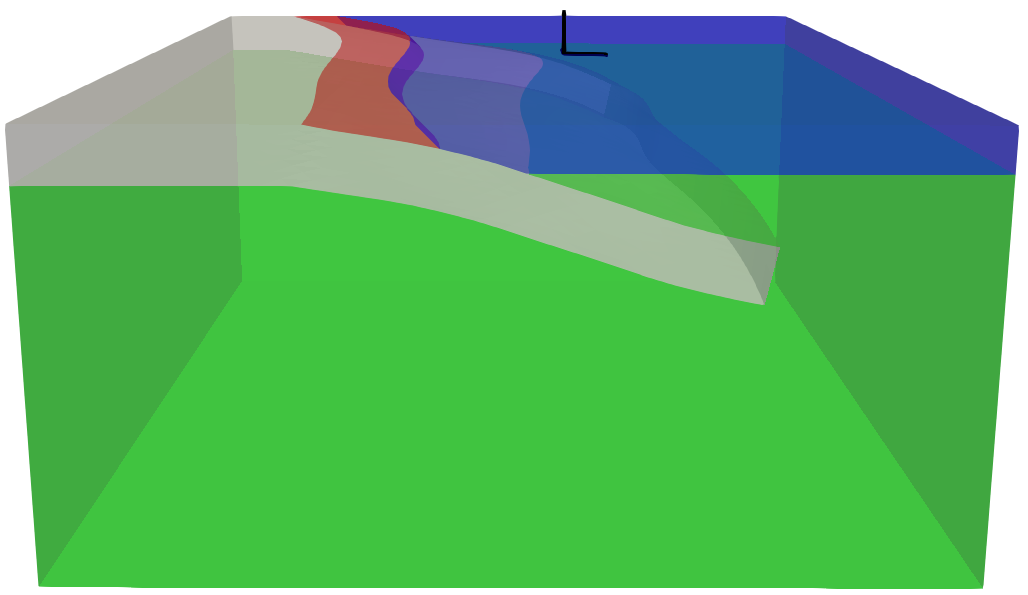
\includegraphics[width=4.5in]{examples/figs/subduction3d_geometry}};
    \begin{scope}[x={(image.south east)},y={(image.north west)}]
      \node[anchor=west, annotation] (xneg) at (-0.2,0.5) {+2.0 m};
      \draw[>=latex, ->, ultra thick, annotation] (xneg) -- (0.0,0.5);
      \node[anchor=east, annotation] (xpos) at (+1.2,0.5) {-2.0 m};
      \draw[>=latex, ->, ultra thick, annotation] (xpos) -- (1.0,0.5);
    \end{scope}
  \end{tikzpicture}
  \caption{Diagram of axial compression example. This static
    simulation uses Dirichlet boundary conditions with axial
    compression in the east-west (x-direction) and purely elastic
    properties.}
  \label{fig:example:subduction:3d:step01:diagram}
\end{figure}

The first example problem is earthquake rupture involving coseismic
slip along the interface between the subducting slab and the continental
crust and uppermost portion of the mantle below the continental crust.
The spatial variation of slip comes from a cross-section of Gavin
Hayes' finite-source model \url{earthquake.usgs.gov/earthquakes/eqinthenews/2011/usc0001xgp/finite_fault.php}.
On the lateral and bottom boundaries of the domain, we fix the degrees
of freedom perpendicular to the boundary as shown in Figure \vref{fig:example:subduction:2d:steps}.
Parameter settings that augment those in \filename{pylithapp.cfg} are
contained in the file \filename{step01.cfg}. These settings are:
\begin{inventory}
  \facilityitem{pylithapp.timedependent.formulation.time\_step}{Adjust the total
    simulation time to 0 years (static simulation).}
  \facilityitem{pylithapp.timedependent}{Specifies the array of
    boundary conditions.}
  \facilityitem{pylithapp.timedependent.bc.\textit{BOUNDARY}}{Defines the settings
    for boundary \textit{BOUNDARY}, including which degrees of freedom
    are being constrained (x or y), the label (defined in\filename{ mesh\_tri3.exo})
    corresponding to the nodeset in CUBIT, and a label to the boundary
    condition used in any error messages.}
  \facilityitem{pylithapp.timedependent.interfaces.fault}{Specify the coseismic
    slip along the interface between the oceanic crust and continental
    crust with a small amount of slip penetrating into the upper mantle.}
  \facilityitem{pylithapp.problem.formulation.output.domain}{Gives the base filenames
    for HDF5 output (for example, \filename{step01.h5}).}
\end{inventory}
We run this example by typing
\begin{shell}
$$ pylith step01.cfg
\end{shell}
The problem will produce twelve pairs of HDF5/Xdmf files. The HDF5
files contain the data and the Xdmf files contain the metadata required
by ParaView and Visit (and possibly other visualization tools that
use Xdmf files) to access the mesh and data sets in the HDF5 files.
The files include the solution over the domain and ground surface
(two pairs of files), physical properties, stress, and strain within
each material (eight pairs of files), and fault parameters, slip,
and traction (two pairs of files). 

Figure \vref{fig:example:subduction:2d:step01}, which was created using
ParaView, displays the magnitude of the displacement field with the
deformation exaggerated by a factor of 1000. 

\begin{figure}
  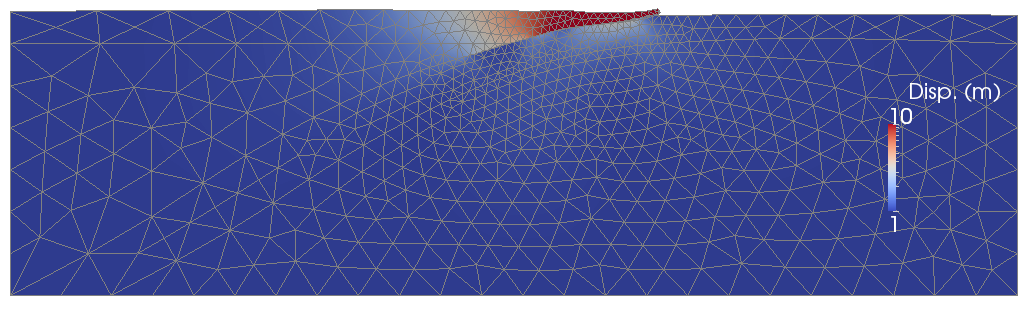
\includegraphics[width=4.5in]{examples/figs/subduction2d_step01_soln}
  \caption{Solution for Step 1. The colors indicate the magnitude of the displacement,
    and the deformation is exaggerated by a factor of 1000. }
  \label{fig:example:subduction:2d:step01}
\end{figure}


\subsubsection{Exercises}

% Algebraic multigrid preconditioner
% Adjust material properties (stiffer, softer, nearly incompressible)
% Pure shear instead of axial compression

\subsection{Step 2: Postseismic Relaxation}

\subsubsection{Exercises}

% Change slip on slab to slip on splay fault
% Slip on lower slab and splay fault
% Slip on slab and splay fault

\subsection{Step 3: Interseismic Deformation}

\subsubsection{Exercises}

\subsection{Step 4: Prescribed Earthquake Cycle}

\subsubsection{Exercises}

% Make lower slab + splay fault the primary fault surface and the
% upper slab (trench side of the splay fault) the secondary fault
% surface. Hint: You will need to create a nodesets in CUBIT that
% correspond to the primary and secondary fault surfaces.



\subsection{Step 5: Spontaneous Rupture Driven by Subducting Slab}

\subsubsection{Exercises}

\subsection{Step 6: Prescribed Slow-Slip Event}

This example simulates a simple slow slip event (SSE) that remains
fixed spatially but increases its amplitude with time. We assume a
constant rake angle of 110 degrees, and a time duration of 30
days. This problem requres the use of both a spatial database to
provide the spatial distribution of slip, and a temporal database to
describe the time evolution of slip. To create these databases we
provide the \filename{generate\_slowslip.py} script, which is in the
\filename{spatialdb} directory. Once you are in the
\filename{spatialdb} directory, run the script as follows:
\begin{shell}
$$ ./generate_slowslip.py
\end{shell}
This script reads parameters from \filename{generate\_slowslip.cfg} to
generate a Gaussian slip distribution in geographic coordinates, along
with a temporal database providing the slip amplitudes at different
times. The files created are:
\begin{itemize}
\item \filename{fault\_slabtop\_slowslip.spatialdb}: Spatial database
\item \filename{fault\_slabtop\_slowslip.timedb}: Temporal database
\end{itemize}

Once the database files have been generated, it is possible to run the
example. Parameter settings that augment those in pylithapp.cfg are
contained in the file \filename{step06.cfg}. These settings are:
\begin{inventory}
  \facilityitem{pylithapp.timedependent.formulation.time\_step}{Adjust
    the total simulation time to 30 days with a time step size of 2 days.}
  \facilityitem{pylithapp.timedependent.formulation}{Specify output
    for the domain, for the ground surface, and for a set of
    simulated cGPS sites.}
  \facilityitem{pylithapp.timedependent.interfaces.slab}{Specify the
    spatial distribution of slip and the temporal evolution of slip on
    the slab interface. We change the slip function from the default
    to a time history slip function to make use of the temporal database.}
  \facilityitem{pylithapp.problem.formulation.output.domain}{Gives the
    base filenames for HDF5 output for all output types (for example, 
    \filename{step06-domain.h5}). Note that for cGPS output we need to
    provide coordinate system information as well as the name of a
    text file providing cGPS site locations.}
\end{inventory}
We use elastic properties for all materials, and custom solver
settings appropriate for a problem with a fault. We run the example by typing
\begin{shell}
$$ pylith step06.cfg mat_elastic.cfg solver_fieldsplit.cfg
\end{shell}
The problem will produce 13 pairs of HDF5/Xdmf files. In the data
files (those without a \filename{\_info} before the file suffix) there
are field values representing 15 time steps. The additional HDF5 file
that was not present in previous examples is
\filename{step06-cgps\_sites.h5}, which contains the displacements at
the simulated cGPS sites.

Figure \vref{fig:example:subduction:3d:step06}, which was created
using ParaView, shows the surface vertical displacement along with
horizontal displacement vectors at the cGPS sites, superimposed on
contours of the applied slip at t = 24 days.

\begin{figure}
  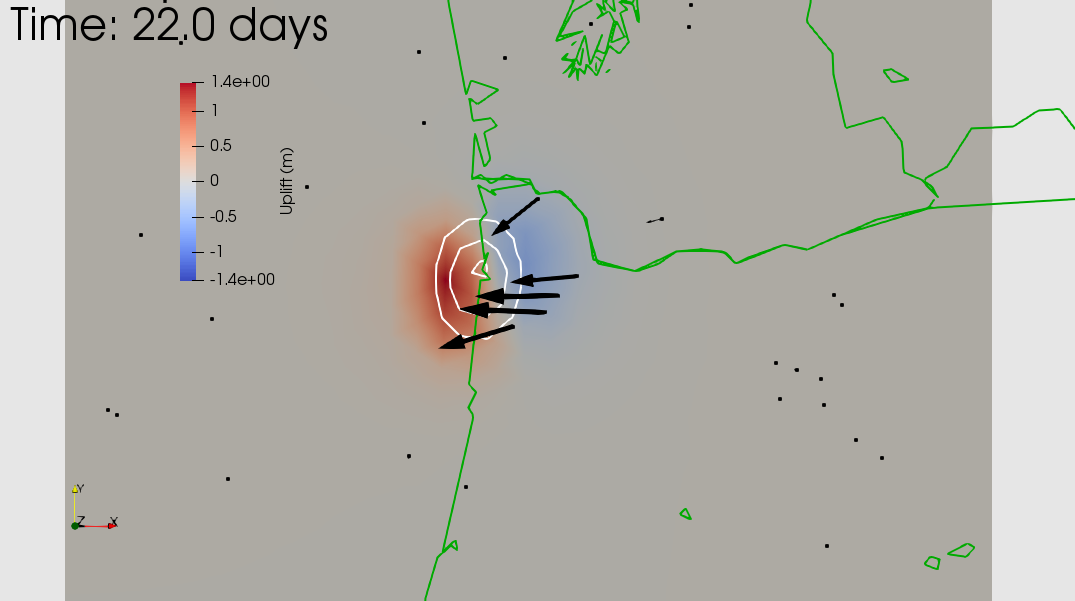
\includegraphics[width=4.5in]{examples/figs/subduction3d_step06_soln}
  \caption{Solution for Step 6. The colors indicate the vertical
    displacement, the vectors represent the horizontal displacements
    at simulated cGPS sites, and the contours represent the applied
    slip at t = 24 days. }
  \label{fig:example:subduction:3d:step06}
\end{figure}


\subsubsection{Exercises}

\begin{itemize}
\item Change spatial distribution and time history of slip.
  \begin{itemize}
  \item Edit \filename{generate\_slowslip.cfg} to change spatial and
    temporal distributions, and edit \filename{step06.cfg} to change the
    time duration and/or time step size.
  \end{itemize}
\item Add propagation of the slow slip (spatial variation of slip
  initiation time).
  \begin{itemize}
  \item Either alter Python script to produce a spatial database of
    slip initiation times, or write a new script.
  \end{itemize}
\end{itemize}

\subsection{Step 7: Inversion of Slow-Slip using 3D Green's Functions}

This example is essentially a three-dimensional analog of
{sec:example:greensfns2d}, and is a more realistic example of how
PyLith can be used to perform geodetic inversions. We use the output
of example step06 to create synthetic data. Once we have done this we
generate Green's functions to represent the geodetic responses at a
set of synthetic cGPS stations. Finally, we use the synthetic data and
Green's functions to perform an inversion, using the same generalized
inverse approach described in {sec:example:greensfns2d}.

We first generate the synthetic data by using the script
\filename{make_synthetic_gpsdisp.py} in the top-level directory. This
script reads the parameters in \filename{make_synthetic_gpsdisp.cfg}
to generate synthetic data from the selected time step with a
specified amount of noise. Run this script as:
\begin{shell}
$$ ./make_synthetic_gpsdisp.py
\end{shell}
This will create the following files:
\begin{itemize}
\item \filename{cgps_synthetic_displacement.txt}: Read by the
  inversion script.
\item \filename{cgps_synthetic_displacement.vtk}: For visualization.
\end{itemize}

After we generate the synthetic data, we generate the Green's
functions. We divide the Green's function generation into two sub-problems:
\begin{itemize}
 \item step07a:  Generate Green's functions corresponding to
   left-lateral slip on the subduction interface (slab top).
 \item step07b:  Generate Green's functions corresponding to
   updip slip on the subduction interface (slab top).
\end{itemize}
Note that the Green's functions could all be generated at the same
time; however, for real problems it is generally preferable to
separate the problems to improve runtimes (e.g., both problems can be
run simultaneously).

To generate the Green's functions we change the problem type from the
default \facility{timedependent} to \facility{greensfns}. We do this
on the command line. When we change the problem type to
\facility{greensfns}, PyLith automatically reads the file
\filename{greensfns.cfg}. We use this file to augment the settings in
\filename{pylithapp.cfg}:


 %% After generating the synthetic data and Green's functions, we then
 %% perform a simple inversion using the slip_invert.py script, with
 %% parameters defined in slip_invert.cfg:

 %% ./slip_invert.py

 %% This will generate two HDF files that may be viewed in Paraview:
 %% step07-inversion-slip.h5:  The predicted fault slip.
 %% step07-inversion-displacement.h5:  The predicted surface displacements.

 %% There is also an inversion summary file:  step07-inversion-summary.txt
 %% If you have matplotlib installed, you can view a log-log plot of
 %% solution misfit by going into the viz directory and running:

 %% ./plot_inversion_misfit.py --summary=../step07-inversion-summary.txt


\subsubsection{Exercises}

% Move slip to splay fault in step06 and redo inversion.
% Adjust noise level
% Invert for slip at each time step

\subsection{Step 8: Gravitational Body Forces}


% End of file
